\documentclass[a4paper,12pt]{report}
% safe参数解决与\!在内的多个冲突
% \sups命令可能被重定义,xeCJK放在tipa后
\usepackage[safe]{tipa}

% 中文支持
\usepackage[slantfont,boldfont]{xeCJK}
	\setCJKmainfont[BoldFont=SimHei,ItalicFont=KaiTi]{SimSun}
	\setCJKmathfont{STXinwei}
\usepackage{indentfirst}

% 数学环境
\usepackage{amsmath}
  \newcommand{\ue}{\mathrm{e}}
  \newcommand{\ud}{\mathop{}\negthinspace\mathrm{d}}
\usepackage{amssymb}
\usepackage{mathrsfs} % 线性代数字体
    % overline的替代命令
\newcommand{\closure}[2][3]{{}\mkern#1mu\overline{\mkern-#1mu#2}}
\usepackage{yhmath} % 左下-右上省略号
\usepackage{mathtools} % dcases环境
\usepackage{amsthm} % 定理环境
  \theoremstyle{definition}\newtheorem{laws}{Law}[section]
  \theoremstyle{plain}\newtheorem{ju}[laws]{Jury}
  \theoremstyle{remark}\newtheorem*{marg}{Margaret}
\usepackage{esint} % 多重积分,需放在amsmath后

% 下划线宏包
\usepackage{ulem}
% LaTeX符号宏包
\usepackage{hologo}
	\newcommand{\xelatex}{\Hologo{XeLaTeX}}
	\newcommand{\bibtex}{\Hologo{BibTeX}}
% 其他符号
\usepackage{wasysym}
% 带箱小页
\usepackage{boxedminipage}
% 绘图
\usepackage{tikz}
	\usetikzlibrary{calc}
	\newcommand{\tikzline}[1]{{#1\tikz{\draw[#1,line width=9](0,0)--(0.5,0);}}, }

% 奇怪的小定义
\newcommand{\dpar}{\\ \mbox{}}	% 空两行
\newcommand{\qd}[1]{{\bfseries{#1}}}	% 强调
\newcommand{\co}[1]{{\bfseries{#1}}}   % Style of concept
\newcommand{\RED}[1]{{\color{red}{#1}}}
\newcommand{\cmmd}[1]{\fbox{\texttt{\char92{}#1}}}
\newcommand{\charef}[1]{第\ref{#1}章}
\newcommand{\secref}[1]{第\ref{#1}节}
\newcommand{\pref}[1]{第\pageref{#1}页}
\newcommand{\fref}[1]{图\ref{#1}}
\newcommand{\tref}[1]{表\ref{#1}}

% 编号列表宏包,并自定义了三个列表
%\usepackage[inline]{enumitem}
%	\setlist[enumerate]{label=\arabic* - ,font=\bfseries,itemsep=0pt}
%	\setlist[itemize]{label=$\bullet$,font=\bfseries,leftmargin=\parindent}
%	\setlist[description]{font=\bfseries\uline}
%
%\newenvironment{fead}{\setlength{\parskip}{0pt}
%	\begin{description}[font=\bfseries\uline,labelindent=\parindent]
%		\setlength{\itemsep}{0pt}\setlength{\parsep}{0pt}\setlength{\parskip}{0pt}}
%	{\end{description}}
% 带宽度的
\newenvironment{para}{\setlength{\parskip}{0pt}
	\begin{description}[font=\bfseries\ttfamily]
		\setlength{\itemsep}{0pt}\setlength{\parsep}{0pt}\setlength{\parskip}{0pt}}
	{\end{description}}
\newenvironment{feae}{\setlength{\parskip}{0pt}
	\begin{enumerate}[font=\bfseries,labelindent=0pt]}
	{\end{enumerate}}
\newenvironment{feai}{\setlength{\parskip}{0pt}
	\begin{itemize}[font=\bfseries]
		\setlength{\itemsep}{0pt}\setlength{\parsep}{0pt}\setlength{\parskip}{0pt}}
	{\end{itemize}}
\newenvironment{inlinee}
{\begin{enumerate*}[label=(\arabic*), font=\rmfamily, before=\unskip{:},itemjoin={{;}},itemjoin*={{,以及:}}]}
	{\end{enumerate*}。}

% 目录和章节样式
\usepackage{titlesec}
\usepackage{titletoc}   % 用于目录

\titlecontents{chapter}[1.5em]{}
	{\contentslabel{1.5em}}{\hspace*{-2em}}{\hfill\contentspage}
	
\titlecontents{section}[3.3em]{}
	{\contentslabel{1.8em}}
	{\hspace*{-2.3em}}
	{\titlerule*[8pt]{$\cdot$}\contentspage}
%	
\titlecontents{subsection}[2.5em]{\small}
	{\thecontentslabel{} }
	{}
	{\titlerule*[5pt]{$\cdot$}\contentspage}
 %章节样式
\setcounter{secnumdepth}{3} % 一直到subsubsection
\newcommand{\chaformat}[1]{%
	\parbox[b]{.5\textwidth}{\hfill\bfseries #1}%
	\quad\rule[-12pt]{2pt}{70pt}\quad
	{\fontsize{60}{60}\selectfont\thechapter}}
\titleformat{\chapter}[block]{\hfill\LARGE\sffamily}{}{0pt}{\chaformat}[\vspace{2.5pc}\large
	\startcontents\printcontents{}{1}{\setcounter{tocdepth}{2}}]
%\titleclass{\section}{top}
%\titleformat{\section}{\Large\bfseries}{\thesection}{0.5em}{}
\titleformat*{\section}{\centering\Large\bfseries}
\titleformat{\subsubsection}[hang]{\bfseries\large}{\rule{1.5ex}{1.5ex}}{0.5em}{}
% 扩展章节
\newcommand{\starsec}{\noindent\fbox{\S\textit{注意:本章节是一个扩展阅读章节。}}
	\\ \mbox{}}

\renewcommand{\contentsname}{目录}
	\renewcommand{\tablename}{表}
	\renewcommand\arraystretch{1.2}	% 表格行距
	\renewcommand{\figurename}{图}
% 设置不需要浮动体的表格和图像标题
\setlength{\abovecaptionskip}{5pt}
\setlength{\belowcaptionskip}{3pt}
\makeatletter
\newcommand\figcaption{\def\@captype{figure}\caption}
\newcommand\tabcaption{\def\@captype{table}\caption}
\makeatother
% 图表
\usepackage{array,multirow}
  \setlength\extrarowheight{2pt} % 行高增加
\usepackage{longtable}
\usepackage{graphicx}
  \graphicspath{{./tikz/}}
% 页面修正宏包
\usepackage[top=1in]{geometry}

% 代码环境
\usepackage{listings}
% Avoid copy line numbers of the listing code (Invalid for SumatraPDF Reader)
\usepackage{accsupp}
	\newcommand{\emptyaccsupp}[1]{\BeginAccSupp{ActualText={}}#1\EndAccSupp{}}
% Color
\usepackage{xcolor}
	\definecolor{commentcolor}{RGB}{85,139,78}
	\definecolor{numbercolor}{RGB}{166,206,168}
	\definecolor{stringcolor}{RGB}{206,145,108}
	\definecolor{keywordcolor}{RGB}{34,34,250}
	\definecolor{backcolor}{RGB}{220,220,220}
	\definecolor{packagecolor}{RGB}{0,128,0}
	\definecolor{envicolor}{RGB}{185,70,15}
% LaTeX Code Style
%\lstset{language=[LaTeX]TeX,
%		basicstyle=\small\ttfamily,
%		commentstyle=\color{commentcolor},
%		keywordstyle=\color{keywordcolor},
%		stringstyle=\color{stringcolor},
%		showstringspaces=false,
%		% Package/Tikz-Lib Using
%		classoffset=0,
%		morekeywords={begin,end,usetikzlibrary},
%		keywordstyle=\color{keywordcolor},
%		classoffset=1,
%		morekeywords={article,report,book,
%			xeCJK,tikz,
%			calc},
%		keywordstyle=\color{packagecolor},
%		classoffset=2,
%		morekeywords={document,tikzpicture},
%		keywordstyle=\color{envicolor},
%		% Line Number Style
%		numbers=left,
%		numberstyle=\tiny\emptyaccsupp,
%		stepnumber=1,
%		% Frame and Background Color
%		frame=single,
%		framerule=0pt,
%		backgroundcolor=\color{backcolor},
%		% Spaces
%		% belowskip=\medskipamount,
%		emptylines=1,
%		escapeinside=``}

\lstnewenvironment{latex}[1]{\lstset{#1}}{}
\newcommand{\latexline}[1]{{\lstinline[language=TeX,basicstyle=\small\ttfamily]{#1}}}

% Tikz Code
\lstdefinelanguage{tikzlang}{
	classoffset=0, % 蓝色的keyword
	morekeywords={begin,end,newcommand,
		draw,node,coordinate,tikzstyle,foreach},
	keywordstyle=\color{keywordcolor},
	classoffset=1, % 棕色的其他关键字
	morekeywords={tikzpicture,grid,at,
		thick,thin,very,ultra,
		red,green,yellow,blue,cyan,magenta,black,
		    gray,darkgray,lightgray,brown,lime,
		    olive,orange,pink,purple,teal,violet,white},
	keywordstyle=\color{envicolor},
	morecomment=[l]{\%},
	morecomment=[s]{/*}{*/},
	morestring=[b]',
	% Escape
	escapeinside=``
}
\lstnewenvironment{tikzcode}[1]{\lstset{language=tikzlang,basicstyle=\small\ttfamily,
		breaklines=true,%backgroundcolor=\color{white},
		linewidth=0.7\linewidth,#1}}{}

% 附录
\usepackage{appendix}

% 行号
\usepackage{lineno}

% 代码输入环境
%\usepackage{verbatim,xcolor}
%\newbox\savedlines
%\newtoks\savedtokens
%\makeatletter
%\def\codeshow{%
%\global\savedtokens={}%
%\def\verbatim@processline{%
%{\setbox0=\hbox{\the\verbatim@line}%
%\hsize=\wd0
%\the\verbatim@line\par}%
%\global\savedtokens=\expandafter{\the\expandafter\savedtokens\the\verbatim@line^^J}}%
%\@tempswatrue
%\setbox0=\vbox\bgroup\parskip=0pt\topsep=0pt\partopsep=0pt
%\verbatim}
%\def\endcodeshow{\endverbatim%
%\unskip\setbox0=\lastbox\egroup
%\global\setbox\savedlines=\box0
%\addvspace{1em}\par\noindent%
%\colorbox{lightgray}{%
%\begin{minipage}{.55\textwidth}{\usebox\savedlines}\end{minipage}}%
%\hfill\fbox{\parbox{.40\textwidth}%
%{\scantokens\expandafter{\the\savedtokens\unskip\endinput}}}%
%\par\addvspace{1em}}
%\makeatother

% 引用
\usepackage[colorlinks,bookmarksopen=true,bookmarksnumbered=true]{hyperref}

\usepackage{algorithm}
\usepackage{amsmath,bm}
\usepackage{algorithmic}
\usepackage{fancybox}
\usepackage{listings}
\usepackage{rotating}
\usepackage{xcolor}
\usepackage{diagbox}
\usepackage{amssymb}
\usepackage{amsmath}
\usepackage{amsthm}
\usepackage{empheq}
\usepackage{warpcol}
\usepackage{lscape}
\usepackage[framemethod=tikz]{mdframed}
\usepackage{mathtools}
\usepackage{longtable,booktabs}

\definecolor{ocre}{RGB}{243,102,25}
\definecolor{mygray}{RGB}{243,243,244}

\newcommand*\mymathbox[1]{%
  \fcolorbox{ocre}{mygray}{\hspace{1em}#1\hspace{1em}}}

\newtheoremstyle{mystyle}
  {\topsep}
  {\topsep}
  {\normalfont}
  {}
  {\sffamily\bfseries}
  {.}
  {.5em}
  {{\color{ocre}\thmname{#1}~\thmnumber{#2}}\thmnote{\,--\,#3}}%
\theoremstyle{mystyle}
\newmdtheoremenv[
  backgroundcolor=mygray,
  linecolor=ocre,
  leftmargin=20pt,
  innerleftmargin=0pt,
  innerrightmargin=0pt,
  ]{theo}{Theorem}[section]

\lstset{
columns=flexible,
numbers=left,
numberstyle=\footnotesize\color{darkgray}, 
basicstyle=\small\ttfamily,
stringstyle=\color{purple},
keywordstyle=\color[RGB]{40,40,255}\bfseries,
commentstyle=\it\color[RGB]{0,96,96},  
stringstyle=\rmfamily\slshape\color[RGB]{128,0,0}, 
showstringspaces=false,      
% directivestyle=\color{blue},
frame=shadowbox,
%framerule=0pt,
backgroundcolor=\color[RGB]{245,245,244},
escapeinside=``, %逃逸字符(1左面的键),用于显示中文
breaklines,
extendedchars=false,
%解决代码跨页时,章节标题,页眉等汉字不显示的问题
xleftmargin=2em,xrightmargin=2em,
aboveskip=1em,%设置边距
tabsize=4, %设置tab空格数  
showspaces=false %不显示空格 
rulesepcolor=\color{red!20!green!20!blue!20}
%rulesepcolor=\color{brown}
}


\title{数值分析第三次大作业}
\author{张晋\\学号:15091060}
\date{最后更新于:\today}
\begin{document}

\maketitle

\tableofcontents


\newpage

\chapter{题目}
关于$x,y,t,u,v,w$的下列方程组:

\[\left\{ \begin{array}{l}
0.5\cos t + u + v + w - x = 2.67\\
t + 0.5\sin u + v + w - y = 1.07\\
0.5t + u + \cos v + w - x = 3.74\\
t + 0.5u + v + \sin w - y = 0.79
\end{array} \right.\]

以及关于$z, t, u$的下列二维数表确定了一个二元函数
$z=f(x,y)$。
\begin{table}[htbp]
  \centering
  \caption{二维数表}
    \begin{tabular}{|>{\centering}p{20pt}|>{\centering}p{40pt}|>{\centering}p{40pt}|>{\centering}p{40pt}|>{\centering}p{40pt}|>{\centering}p{40pt}|>{\centering\arraybackslash}p{40pt}|}
    \hline
    \diagbox{t}{z}{y}& 0     & 0.4   & 0.8   & 1.2   & 1.6   & 2 \\
    \hline
    0     & -0.5  & -0.34 & 0.14  & 0.94  & 2.06  & 3.5 \\
    \hline
    0.2   & -0.42 & -0.5  & -0.26 & 0.3   & 1.18  & 2.38 \\
    \hline
    0.4   & -0.18 & -0.5  & -0.5  & -0.18 & 0.46  & 1.42 \\
    \hline
    0.6   & 0.22  & -0.34 & -0.58 & -0.5  & -0.1  & 0.62 \\
    \hline
    0.8   & 0.78  & -0.02 & -0.5  & -0.66 & -0.5  & -0.02 \\
    \hline
    1     & 1.5   & 0.46  & -0.26 & -0.66 & -0.74 & -0.5 \\
    \hline
    \end{tabular}
  \label{tab:addlabel}
\end{table}

\begin{enumerate}
\item 试用数值方法求出$f(x, y)$在区域
$D = \{ (x,y)|0 \le x \le 0.8,0.5 \le y \le 1.5\}$上的一个近似表达式:
\[p(x,y) = \sum_{r = 0}^k\sum_{s = 0}^k {{c_{rs}}{x^r}{y^s}} \]
要求$p(x,y)$最小的$k$值达到以下的精度:
\[\sigma  = \sum\limits_{i = 0}^{10} {\sum\limits_{j = 0}^{20} {[f({x_i},{y_j}) - p} } ({x_i},{y_j}){]^2} \le {10^{ - 7}}\]
其中,${x_i} = 0.08i,{y_j} = 0.5 + 0.05j$

\item 计算$f(x_i^{\ast},y_j^{\ast}),p(x_i^{\ast},y_j^{\ast})\qquad (i = 1, 2,\cdots,8;j = 1,2,\cdots,5)$的值,以观察$p(x,y)$逼近$f(x,y)$的效果,其中,$x_i^{\ast}=0.1i,y_j^{\ast}=0.5+0.2j$
\end{enumerate}


\subsection*{说明:}
\begin{enumerate}
\item 用迭代方法求解非线性方程组时,要求近似解向量
${\bm{x}^{(k)}}$满足以下精度
\[\dfrac{\|{\bm{x}^{(k)}} - {\bm{x}^{(k - 1)}}\|_{\infty }}{\|{\bm{x}^{(k)}}\|_{\infty }} \le {10^{ - 12}}\]

\item 作二元插值时,要使用分片二次代数插值。

\item 要由程序自动确定最小的$k$值。

\item 打印以下内容:

\begin{enumerate}
\item 全部源程序;

\item 数表:$\{{x_i},{y_j},f({x_i},{y_j})\}\qquad (i = 0,1,2,\cdots,10;j = 0,1,2,\cdots,20)$;

\item 选择过程的$k,\sigma$值;

\item 达到精度要求时的$k$和$\sigma$值以及$p(x,y)$中的系数
$c_{rs}(r = 0,1,\cdots,k;s = 0,1,\cdots,k)$;

\item 数表:$\{x_i^{\ast},y_j^{\ast},f(x_i^{\ast},y_j^{\ast}),p(x_i^{\ast},y_j^{\ast})\}\qquad (i = 1, 2,\cdots,8;j = 1,2,\cdots,5)$。

\end{enumerate}
\item 采用$f$型输出$x_i,y_j,x_i^{\ast},y_j^{\ast}$的准确值,其余实型数采用$e$型输出并且至少显示12位有效数字。
\end{enumerate}


\newpage
\chapter{算法设计方案}
\section{方案综述}
\begin{enumerate}
\item 将${x_i} = 0.08i,{y_j} = 0.5 + 0.05j\quad (i=0,1,\cdots,10;j=0,1,\cdots,20)$代入非线性方程组(\ref{e1})中,用\hyperref[sec:Newton]{Newton迭代法}解出$t_{ij}$和$u_{ij}$;

\item 对数表$z(t,u)$进行\hyperref[sec:Interpolation]{分片双二次插值},求得$z_{ij}=\hat{z}(t_{ij},u_{ij})$

\item 根据$z_{ij}$的值进行\hyperref[sec:qmnh]{曲面拟合},要求精度
$\sigma \le 10^{-7}$
,得拟合函数
\[p(x,y) = \sum_{r = 0}^k\sum_{s = 0}^k {{c_{rs}}{x^r}{y^s}} \]

\item 
创建新的数据点集$x_i^{\ast}=0.1i,y_j^{\ast}=0.5+0.2j\quad (i = 1, 2,\cdots,8;j = 1,2,\cdots,5)$,
并代入非线性方程组(\ref{e1})中,用\hyperref[sec:Newton]{Newton迭代法}解出$t^{\ast}$和$u^{\ast}$,
再用\hyperref[sec:Interpolation]{分片双二次插值}计算出$f(x^{\ast},y^{\ast})$,将其与$p(x^{\ast},y^{\ast})$输出并观察比较。\footnote{算法流程图见第\pageref{flow}页。}
\end{enumerate}




\newpage
\begin{figure}[h]
\small
\centering
\label{flow}
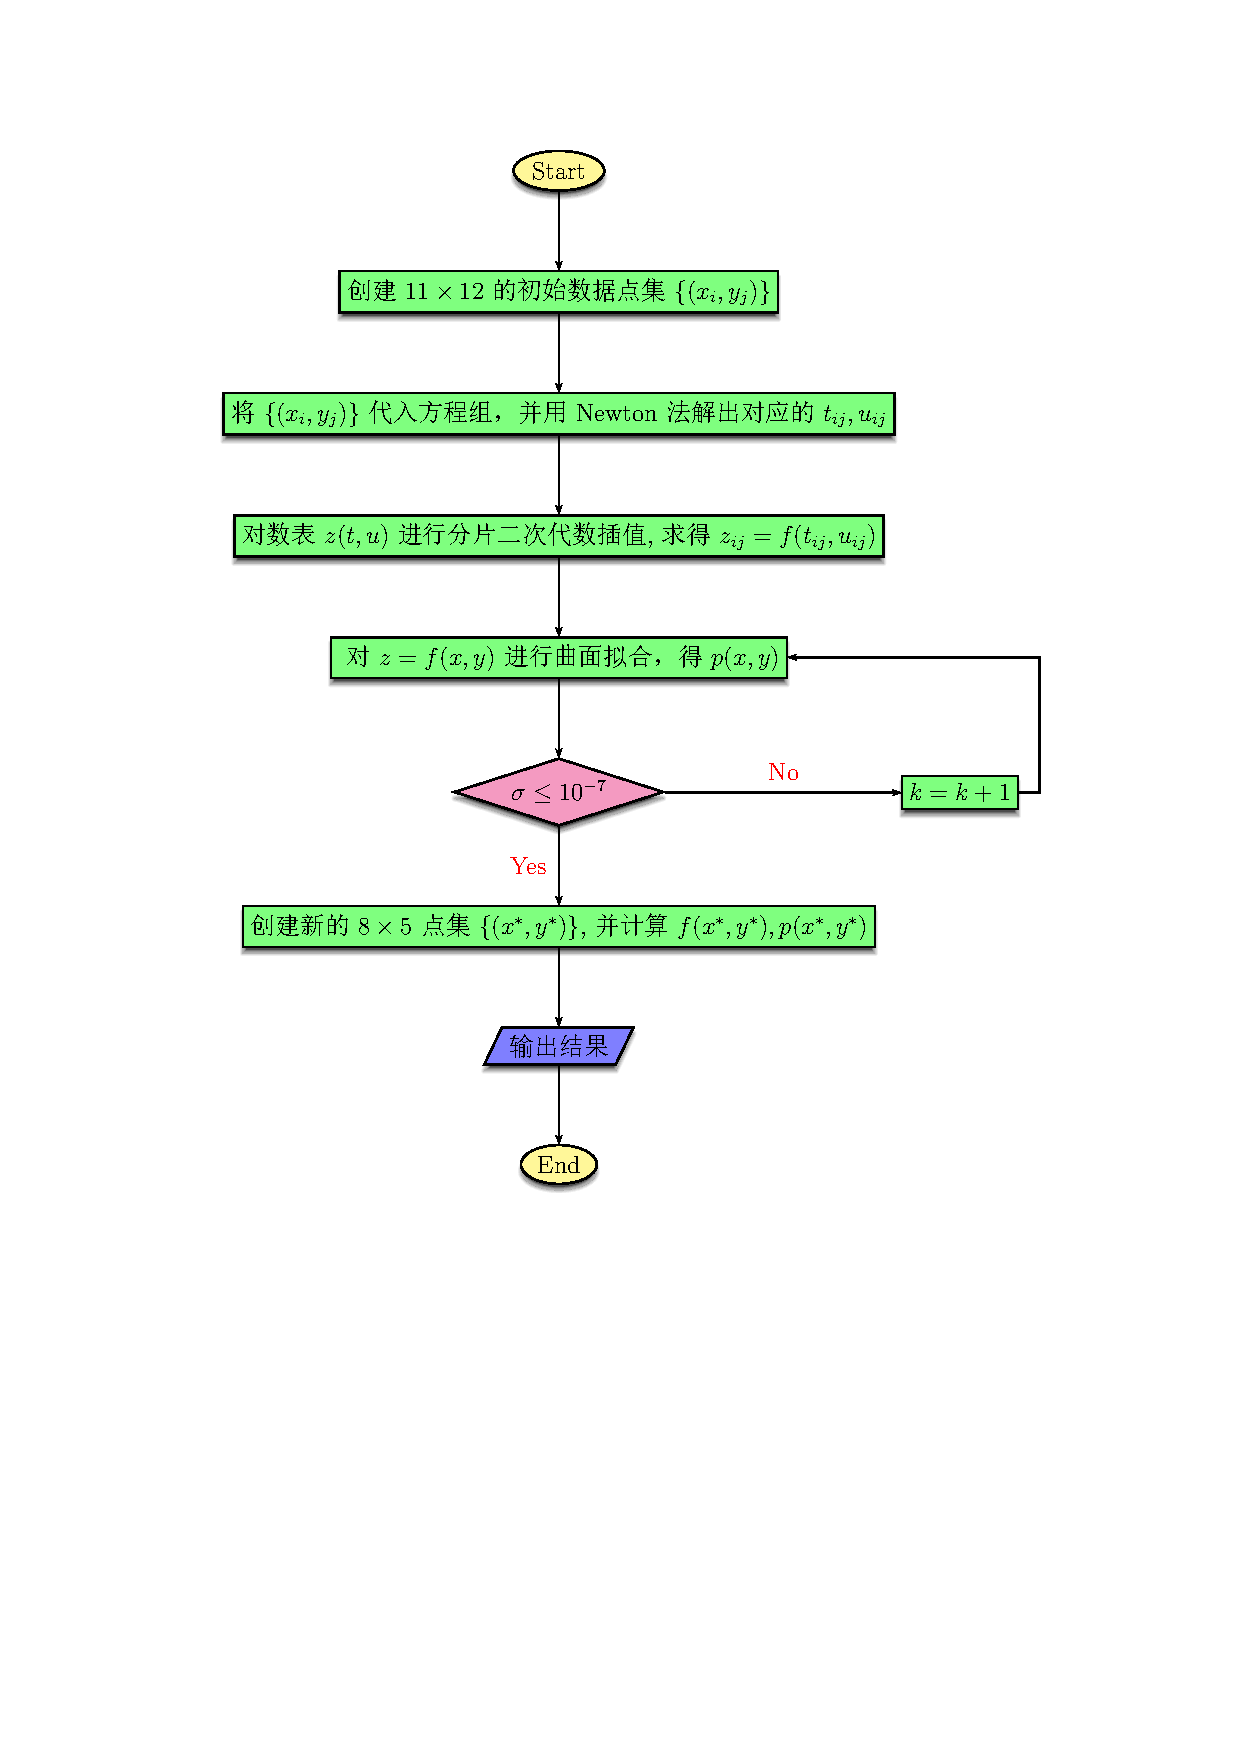
\includegraphics[width=17cm]{flow1}
\end{figure}

\newpage
\section{Newton迭代法}
\label{sec:Newton}
\begin{equation}
\label{e1}
\left\{ \begin{array}{l}
0.5\cos t + u + v + w - x = 2.67\\
t + 0.5\sin u + v + w - y = 1.07\\
0.5t + u + \cos v + w - x = 3.74\\
t + 0.5u + v + \sin w - y = 0.79
\end{array} \right.
\end{equation}


对于该非线性方程组方程组来说,$x,y$为已知量,
需解出$t,u,v,w$。

设$\bm{x}= {(t,u,v,w)^T}$,并设定精度水平${\varepsilon } = {10^{ - 12}}$和最大迭代次数$M$

先在${\bm{x}^{\ast}}$附近选取${\bm{x}^{(0)}}= {({t^{(0)}},{u^{(0)}},{v^{(0)}},{w^{(0)}})^T}$
然后迭代\footnote{迭代的终止条件为$\|\Delta \bm{x}^{(k)}\|/\|\bm{x}^{(k+1)}\|\le \varepsilon$,若$k>M$时仍未达到迭代精度,则迭代失败。}:
\[\bm{x}^{(k+1)}= \bm{x}^{(k)}-[\bm{F}'(\bm{x}^{(k))}]^{-1}\bm{F}(\bm{x}^{(k)})\]
具体算法如下:
\begin{algorithm}[h]  
\caption{Newton's method}  
\begin{algorithmic}[1]  
\STATE Set $\bm{x}^{(0)}\in D$ and $k=0$
\WHILE {k<M}
\STATE Compute $\bm{F}(\bm{x}^{(k)})$ 
and $\bm{F}'(\bm{x}^{(k)})$
\STATE Compute $\Delta \bm{x}^{(k)}=-[\bm{F}'(\bm{x}^{(k))}]^{-1}\bm{F}(\bm{x}^{(k)})$
\IF {$\|\Delta \bm{x}^{(k)}\|/\|\bm{x}^{(k+1)}\|\le \varepsilon$}
\STATE $\bm{x}^{\ast}=\bm{x}^{(k)}$
\STATE \textbf{Break}
\ENDIF 
\STATE $\bm{x}^{(k+1)}= \bm{x}^{(k)}+
\Delta \bm{x}^{(k)}$
\STATE k=k+1
\ENDWHILE
\end{algorithmic}  
\end{algorithm}  

其中,基于方程组(\ref{e1})的$\bm{F}(\bm{x})\text{及其雅可比矩阵}\bm{F}'(\bm{x})$分别为:
\[F(\bm{x}) = \left[ \begin{array}{l}
0.5*cos(t)  +  u  +  v  +  w  -  x  -  2.67\\
t  +  0.5*sin(u)  +  v  +  w  -  y  -  1.07\\
0.5*t  +  u  +  cos(v)  +  w  -  x  -  3.74\\
t  +  0.5*u  +  v  +  sin(w)  -  y  -  0.79
\end{array} \right]\]

\[F'(\bm{x}) = \left[ {\begin{array}{*{20}{c}}
{ - 0.5*\sin (t)}&1&1&1\\
1&{0.5*\cos (u)}&1&1\\
{0.5}&1&{ - \sin (v)}&1\\
1&{0.5}&1&{\cos (w)}
\end{array}} \right]\]


\newpage
\section{分片双二次插值}
\label{sec:Interpolation}
前面我们将$\{(x_i,y_j)\}$代入非线性方程组(\ref{e1})中,然后用\hyperref[sec:Newton]{Newton迭代法}解出了$t_{ij}$和$u_{ij}$.

在这一节中我们需要根据\tref{tab:addlabel}对$z(t,u)$进行分片双二次插值,求得$z_{ij}=\hat{z}(t_{ij},u_{ij})\qquad (i = 0,1,2,\cdots,10;j = 0,1,2,\cdots,20)$.

因为\tref{tab:addlabel}为$6\times 6$的数表,故可设:
\[{t_i} = ih\qquad(i = 0,1, \cdots ,5)\]
\[{u_i} = j\tau\qquad(j = 0,1, \cdots ,5)\footnote{其中:$\quad h = 0.2 ,\tau  = 0.4$}\]

对于给定的$(t,u)$,如果$(t,u)$满足:
\[{t_i} - \dfrac{h}{2} < t \le {t_i} + \dfrac{h}{2},\footnote{计算$i,j$时有个小技巧:可取$i=\lfloor \dfrac{t}{h}+0.5\rfloor $}\qquad2 \le i \le 3\]
\[{u_j} - \frac{\tau }{2} < u \le {u_j} + \frac{\tau }{2},\footnote{同样的,$j=\lfloor \dfrac{u}{\tau}+0.5\rfloor $}\qquad  2 \le j \le 3\]
那么应选择$({t_k},{u_r})\quad(k = i - 1,i,i + 1;r = j - 1,j,j + 1)$为插值节点。

若$t$满足:
\[t \le {t_1} + \frac{h}{2}\]
或
\[t > {t_3} + \frac{h}{2}\]
则相应地选取$i=1$或$i=4$

同样的,若$u$满足:
\[u \le {u_1} + \frac{\tau }{2}\]
或
\[u> {u_3} + \frac{\tau }{2}\]
则相应地选取$j=1$或$j=4$

最后得到插值多项式为

\begin{equation}
\label{hz}
\boxed{
\hat{z}(t,u) = \sum\limits_{k = i - 1}^{i + 1} {\sum\limits_{r = j - 1}^{j + 1} {{l_k}} } (t){\tilde l_r}(u)z({t_k},{u_r}) }
\end{equation}

其中,
\[{l_k}(t) = \prod\limits_{\substack{m= i - 1\\
m \ne k}}^{i + 1} {\frac{{t - {t_m}}}{{{t_k} - {t_m}}}}\qquad (k = i - 1,i,i + 1)\]

\[{{\tilde l}_r}(u) = \prod\limits_{\substack{n = j - 1\\
n \ne r}}^{j + 1} {\frac{{u - {u_n}}}{{{u_r} - {u_n}}}} \qquad (r = j - 1,j,j + 1)\]

\newpage
\section{曲面拟合}
\label{sec:qmnh}
设在三维坐标系$Oxyu$中给定$(m+1)\times (n+1)$个点:
\begin{equation}
\label{data}
\mathfrak{D}=\{(x_i,y_j),z_{ij}\}\qquad (i=0,1,\cdots,m;j=0,1,\cdots,n)
\end{equation}
选定$M+1$个$x$的函数
$\{\varphi_{r}(x)\}_{r=0}^M$
和$N+1$个$y$的函数
$\{\psi_{s}(y)\}_{s=0}^N$

以函数组$\{\varphi_{r}(x)\psi_{s}(y)\}\quad (r=0,1,\cdots,M;s=0,1,\cdots,N)$为基函数,构成以$\{c_{rs}\}$为参数的曲面族
\begin{equation}
\label{qmz}
p(x,y) = \sum_{r = 0}^M \sum_{s = 0}^N c_{rs}\varphi_{r}(x)\psi_{s}(y)
\end{equation}
 
若参数$\{ c^{\ast}_{rs}\}$使得
\begin{equation}
\label{cost}
L(\bm{C})=\sum\limits_{i = 0}^{m} {\sum\limits_{j = 0}^{n} \left[{\sum_{r = 0}^M \sum_{s = 0}^N c_{rs}\varphi_{r}(x_i)\psi_{s}(y_j) - u_{ij}}\right]^2} 
\end{equation}
在$\bm{C}=\bm{C}^{\ast}$处取到最小值$L(\bm{C}^{\ast})$,则称相应曲面$p^{\ast}(x,y)$为在曲面族(\ref{qmz})中按
\textcolor{blue}{最小二乘原则}确定的
对于数据(\ref{data})的拟合曲面。

设:
\[\bm{B} =\big[\varphi_{r}(x_i)\big]_{(m+1)\times (M+1)}\]
\[\bm{G} =\big[\psi_{s}(y_j)\big]_{(n+1)\times (N+1)}\]
\[\bm{U} =\big[u_{ij}\big]_{(m+1)\times (n+1)}\]
\[\bm{C} =\big[c_{rs}\big]_{(M+1)\times (N+1)}\]

可证得\footnote{在\hyperref[sec:discuss]{第五章}的讨论中,本文将给出一种与教材不同的证明方法},拟合曲面的系数矩阵为
\begin{equation}
\label{c}
\bm{C}=(\bm{B}^T\bm{B})^{-1}\bm{B}^T\bm{U}\bm{G}(\bm{G}^T\bm{G})^{-1}
\end{equation}

在本实验中:
\[\bm{B}=
\begin{bmatrix}
1&{x_0}&{x_0}^{2}& \cdots &{x_0}^{k}\\
1&{x_1}&{x_1}^{2}& \cdots &{x_1}^{k}\\
 \vdots & \vdots & \vdots & \ddots & \vdots \\
1&{x_{10}}^2&{x_{10}}^{2}& \cdots &{x_{10}}^{k}\\
\end{bmatrix}_{11\times (k+1)}\]
\[\bm{G}=
\begin{bmatrix}
1&{y_0}&{y_0}^{2}& \cdots &{y_0}^{k}\\
1&{y_1}&{y_1}^{2}& \cdots &{y_1}^{k}\\
 \vdots & \vdots & \vdots & \ddots & \vdots \\
1&{y_{20}}^2&{y_{20}}^{2}& \cdots &{y_{20}}^{k}\\
\end{bmatrix}_{21\times (k+1)}\]

\[\bm{U} =
\big[u_{ij}\big]_{(m+1)\times (M+1)}=
\big[z_{ij}\big]_{11\times 21}=
\big[f(x_i,y_j)\big]_{11\times 21}
\]

在计算(\ref{c})式时,需要求矩阵的逆,此处可采用Gauss消元法。

解出$c_{rs}^{k}$后,可得:
\[p^{(k)}(x,y) = \sum\limits_{r,s = 0}^k {{c_{rs}^{k}}{x^r}{y^s}} \]



其算法如下:\footnote{写成这样的矩阵形式能有更直观的理解,详细请参看\hyperref[sec:discuss]{第五章}}

\begin{algorithm}[h]  
\caption{Surface Fitting }  
\begin{algorithmic}[1]  
\STATE Set $k=0,\sigma=1$
\WHILE {$\sigma >\varepsilon$}
\STATE Compute $\bm{C}=(\bm{B}^T\bm{B})^{-1}\bm{B}^T\bm{U}\bm{G}(\bm{G}^T\bm{G})^{-1}$ 
\STATE Compute $\bm{P}=\bm{B}\bm{C}\bm{G}^T$ 
\STATE Compute $\sigma={\|{\bm{P}-\bm{U}}\|_{E}^2}$
\STATE k=k+1
\IF {$k>N$}
\STATE \textbf{Break}
\ENDIF 
\ENDWHILE
\end{algorithmic}  
\end{algorithm}  

\newpage



\chapter{源程序}
\begin{lstlisting}[language=C]
#include<stdio.h>
#include<math.h>
#include<string.h>
#define N 100
double X[N];//t,u,v,w 
void F(double x,double y,double Fx[N]){
	Fx[1]=0.5*cos(X[1])+X[2]+X[3]+X[4]-x-2.67;
	Fx[2]=X[1]+0.5*sin(X[2])+X[3]+X[4]-y-1.07;
	Fx[3]=0.5*(X[1])+X[2]+cos(X[3])+X[4]-x-3.74;
	Fx[4]=X[1]+0.5*X[2]+X[3]+sin(X[4])-y-0.79;
}

void JF(double x,double y,double A[N][N]){
	A[1][1]=-0.5*sin(X[1]);	A[1][2]=1;	A[1][3]=1;	A[1][4]=1;
	A[2][1]=1;	A[2][2]=0.5*cos(X[2]);	A[2][3]=1;	A[2][4]=1;
	A[3][1]=0.5;A[3][2]=1;	A[3][3]=-sin(X[3]);		A[3][4]=1;
	A[4][1]=1;	A[4][2]=0.5;	A[4][3]=1;	A[4][4]=cos(X[4]);
}

void clear(double a[N][N]){
	for(int i=0;i<N;i++)
		for(int j=0;j<N;j++)
			a[i][j]=0;
}

void put(double a[N][N],int n,int m){
	for(int i=1;i<=n;i++){
		for(int j=1;j<=m;j++)
			printf("C[%d][%d]=%.12e \n",i-1,j-1,a[i][j]);
		printf("\n");
	}
	printf("\n");
}

double Maxtrix_x(double a[N][N],double b[N][N],double c[N][N],int m,int p,int n){
	double s=0;
	clear(c);
	for(int i=1;i<=m;i++)
		for(int j=1;j<=n;j++)
			for(int k=1;k<=p;k++)
				c[i][j]+=a[i][k]*b[k][j];
}

void Inverse(double C[N][N],double B[N][N],double n){
	double m,A[N][N];
	clear(B);
	clear(A);
	for(int i=1;i<=n;i++)
		for(int j=1;j<=n;j++)
			A[i][j]=C[i][j];
	for(int k=1;k<=n;k++)B[k][k]=1;
	for(int k=1;k<n;k++){
		for(int i=k+1;i<=n;i++){
			m=A[i][k]/A[k][k];
			for(int j=1;j<=n;j++){
				A[i][j]-=m*A[k][j];
				B[i][j]-=m*B[k][j];
			}
		}
	} 
	for(int k=n;k;k--){
		for(int i=n;i>k;i--){
			m=A[k][i];
			for(int j=1;j<=n;j++){
				A[k][j]-=m*A[i][j];
				B[k][j]-=m*B[i][j];
			}
		}
		m=A[k][k];
		for(int j=1;j<=n;j++){
			A[k][j]/=m;
			B[k][j]/=m;
		}
	}
}

void Transpose(double A[N][N],double B[N][N],int n,int m){
	clear(B);
	for(int i=1;i<=n;i++)
		for(int j=1;j<=m;j++)
			B[j][i]=A[i][j];
}

double MaxX(double x[N],int n){
	double max=0;
	for(int i=1;i<=n;i++)
		if(fabs(x[i])>max)max=fabs(x[i]);
}

void Newton(double x,double y){
	int n=4,k;
	double eps=1e-12,max,A[N][N],Fx[N],B[N][N],dX[N];
	for(k=1;k<=1000;k++){
		memset(Fx,0,sizeof(Fx));
		memset(B,0,sizeof(B));
		memset(dX,0,sizeof(dX));
		F(x, y, Fx);
		JF(x, y, A);
		Inverse(A,B,n);
		for(int i=1;i<=n;i++)
			for(int j=1;j<=n;j++)
				dX[i]+=Fx[j]*B[i][j];
		max=0;
		for(int i=1;i<=n;i++)
			if(fabs(X[i])>max)max=fabs(X[i]);
		if((MaxX(dX,n)/max)<eps)
			return ;
		for(int i=1;i<=n;i++)X[i]-=dX[i];
	}
//	printf("wrong!\n");
}

double Interpolation(double t,double u){
	double h=0.2,tau=0.4;
	double z[N][N],sum=0,p;
	int i,j;
z[0][0]=-0.5 ; z[0][1]=-0.34; z[0][2]= 0.14; z[0][3]= 0.94; z[0][4]= 2.06;  z[0][5]= 3.5;
z[1][0]=-0.42; z[1][1]=-0.5 ; z[1][2]=-0.26; z[1][3]= 0.3 ; z[1][4]= 1.18;  z[1][5]= 2.38;
z[2][0]=-0.18; z[2][1]=-0.5 ; z[2][2]=-0.5 ; z[2][3]=-0.18; z[2][4]= 0.46;  z[2][5]= 1.42;
z[3][0]= 0.22; z[3][1]=-0.34; z[3][2]=-0.58; z[3][3]=-0.5 ; z[3][4]=-0.1 ;  z[3][5]= 0.62;
z[4][0]= 0.78; z[4][1]=-0.02; z[4][2]=-0.5 ; z[4][3]=-0.66; z[4][4]=-0.5 ;  z[4][5]=-0.02;
z[5][0]= 1.5 ; z[5][1]= 0.46; z[5][2]=-0.26; z[5][3]=-0.66; z[5][4]=-0.74;  z[5][5]=-0.5; 
	if(t<0.3)i=1;
	else if(t>0.7)i=4;
	else if(0.3<=t && t<=0.7)i=int(t/h+0.5);
	if(u<0.6)j=1;
	else if(u>1.4)j=4;
	else if(0.6<=u && u<=1.4)j=int(u/tau+0.5);

	for(int k=i-1;k<=i+1;k++)
		for(int r=j-1;r<=j+1;r++){
			p=1;
			for(int m=i-1;m<=i+1;m++){
				if(m==k)continue;
				p*=(t-h*m)/(h*k-h*m);
			}
			for(int n=j-1;n<=j+1;n++){
				if(n==r)continue;
				p*=(u-tau*n)/(tau*r-tau*n);
			}
			p*=z[k][r];
			sum+=p;
		}
	return sum;
}

double Surface_Fitting(double x[N],double y[N],double z[N][N],double C[N][N],int k){
	double B[N][N],G[N][N],I[N][N],J[N][N],sigma=0;
	for(int i=1;i<=11;i++)
		for(int j=1;j<=k+1;j++)
			B[i][j]=pow(x[i],j-1);
	for(int i=1;i<=21;i++)
		for(int j=1;j<=k+1;j++)
			G[i][j]=pow(y[i],j-1);

	Transpose(B,I,11,k+1);	
	Maxtrix_x(I,B,J,k+1,11,k+1);
	Inverse(J,C,k+1);
	Maxtrix_x(C,I,J,k+1,k+1,11);
	Maxtrix_x(J,z,I,k+1,11,21);
	Maxtrix_x(I,G,J,k+1,21,k+1);
	Transpose(G,I,21,k+1);
	Maxtrix_x(I,G,C,k+1,21,k+1);
	Inverse(C,I,k+1);
	Maxtrix_x(J,I,C,k+1,k+1,k+1);	
	
	Maxtrix_x(B,C,I,11,k+1,k+1);
	Transpose(G,J,21,k+1);
	Maxtrix_x(I,J,G,11,k+1,21);
	for(int i=1;i<=11;i++)
		for(int j=1;j<=21;j++)
		 sigma+=(G[i][j]-z[i][j])*(G[i][j]-z[i][j]);
	return sigma;
}

int	main(){
	freopen("Work.out","w",stdout);
	double x[N],y[N],Z[N][N],C[N][N],sigma,eps=1e-7;
	int k;
	for(int i=0;i<=10;i++)
		for(int j=0;j<=20;j++){
			x[i+1]=0.08*i;
			y[j+1]=0.5+0.05*j;
			for(int k=1;k<=4;k++)X[k]=1;
			Newton(x[i+1],y[j+1]);
			Z[i+1][j+1]=Interpolation(X[1],X[2]);
			printf("x[%d]=%lf  y[%d]=%lf  f(x,y)=%.12e \n",i,x[i+1],j,y[j+1],Z[i+1][j+1]);
		}
	for(k=0;k<=10;k++){
		sigma=Surface_Fitting(x,y,Z,C,k);
		printf("K=%d,sigma=%.12e\n",k,sigma);
		if(fabs(sigma)<eps)break;
	}
	put(C,k+1,k+1);

	sigma=0;
	for(int i=1;i<=8;i++)
	for(int j=1;j<=5;j++){
		x[i]=0.1*i;
		y[j]=0.5+0.2*j;
		for(k=1;k<=4;k++)X[k]=1;
		Newton(x[i],y[j]);
		sigma=Interpolation(X[1],X[2]);
		printf("x[%d]=%lf  y[%d]=%lf  f(x,y)=%.12e ",i,x[i],j,y[j],sigma);
		sigma=0;
		for(int r=0;r<=k;r++)
		for(int s=0;s<=k;s++){
			sigma+=C[r+1][s+1]*pow(x[i],r)*pow(y[j],s);
		}
		printf("f(x,y)=%.12e\n",i,j,sigma);
		
		
	}
	
	return 0;
}


\end{lstlisting}




\chapter{计算结果}

\begin{longtable}{ccc}

\toprule
 $x_i$ & $y_j$ & $f(x_i,y_j)$\\
\midrule
\endhead

\caption{数表${x_i},{y_j},f({x_i},{y_j})$}\\
\toprule
 $x_i$ & $y_j$ & $f(x_i,y_j)$\\
 \midrule
\endfirsthead
\bottomrule
\endfoot
\bottomrule
\endlastfoot
$x_{0}=$0.000000 & $y_{0}=$0.500000 & $f(x_{0},y_{0})=$4.465040184807e-001 \\
$x_{0}=$0.000000 & $y_{1}=$0.550000 & $f(x_{0},y_{1})=$3.246832629277e-001 \\
$x_{0}=$0.000000 & $y_{2}=$0.600000 & $f(x_{0},y_{2})=$2.101596866827e-001 \\
$x_{0}=$0.000000 & $y_{3}=$0.650000 & $f(x_{0},y_{3})=$1.030436083160e-001 \\
$x_{0}=$0.000000 & $y_{4}=$0.700000 & $f(x_{0},y_{4})=$3.401895562676e-003 \\
$x_{0}=$0.000000 & $y_{5}=$0.750000 & $f(x_{0},y_{5})=$-8.873581363800e-002 \\
$x_{0}=$0.000000 & $y_{6}=$0.800000 & $f(x_{0},y_{6})=$-1.733716327497e-001 \\
$x_{0}=$0.000000 & $y_{7}=$0.850000 & $f(x_{0},y_{7})=$-2.505346114666e-001 \\
$x_{0}=$0.000000 & $y_{8}=$0.900000 & $f(x_{0},y_{8})=$-3.202765063876e-001 \\
$x_{0}=$0.000000 & $y_{9}=$0.950000 & $f(x_{0},y_{9})=$-3.826680661097e-001 \\
$x_{0}=$0.000000 & $y_{10}=$1.000000 & $f(x_{0},y_{10})=$-4.377957667384e-001 \\
$x_{0}=$0.000000 & $y_{11}=$1.050000 & $f(x_{0},y_{11})=$-4.857589414438e-001 \\
$x_{0}=$0.000000 & $y_{12}=$1.100000 & $f(x_{0},y_{12})=$-5.266672548835e-001 \\
$x_{0}=$0.000000 & $y_{13}=$1.150000 & $f(x_{0},y_{13})=$-5.606384797965e-001 \\
$x_{0}=$0.000000 & $y_{14}=$1.200000 & $f(x_{0},y_{14})=$-5.877965387677e-001 \\
$x_{0}=$0.000000 & $y_{15}=$1.250000 & $f(x_{0},y_{15})=$-6.082697790899e-001 \\
$x_{0}=$0.000000 & $y_{16}=$1.300000 & $f(x_{0},y_{16})=$-6.221894528764e-001 \\
$x_{0}=$0.000000 & $y_{17}=$1.350000 & $f(x_{0},y_{17})=$-6.296883781856e-001 \\
$x_{0}=$0.000000 & $y_{18}=$1.400000 & $f(x_{0},y_{18})=$-6.308997600028e-001 \\
$x_{0}=$0.000000 & $y_{19}=$1.450000 & $f(x_{0},y_{19})=$-6.259561525454e-001 \\
$x_{0}=$0.000000 & $y_{20}=$1.500000 & $f(x_{0},y_{20})=$-6.149885466094e-001 \\
$x_{1}=$0.080000 & $y_{0}=$0.500000 & $f(x_{1},y_{0})=$6.380152265113e-001 \\
$x_{1}=$0.080000 & $y_{1}=$0.550000 & $f(x_{1},y_{1})=$5.066117551467e-001 \\
$x_{1}=$0.080000 & $y_{2}=$0.600000 & $f(x_{1},y_{2})=$3.821763692774e-001 \\
$x_{1}=$0.080000 & $y_{3}=$0.650000 & $f(x_{1},y_{3})=$2.648634911537e-001 \\
$x_{1}=$0.080000 & $y_{4}=$0.700000 & $f(x_{1},y_{4})=$1.547802002848e-001 \\
$x_{1}=$0.080000 & $y_{5}=$0.750000 & $f(x_{1},y_{5})=$5.199268349094e-002 \\
$x_{1}=$0.080000 & $y_{6}=$0.800000 & $f(x_{1},y_{6})=$-4.346804020491e-002 \\
$x_{1}=$0.080000 & $y_{7}=$0.850000 & $f(x_{1},y_{7})=$-1.316010567885e-001 \\
$x_{1}=$0.080000 & $y_{8}=$0.900000 & $f(x_{1},y_{8})=$-2.124310883088e-001 \\
$x_{1}=$0.080000 & $y_{9}=$0.950000 & $f(x_{1},y_{9})=$-2.860045510580e-001 \\
$x_{1}=$0.080000 & $y_{10}=$1.000000 & $f(x_{1},y_{10})=$-3.523860789794e-001 \\
$x_{1}=$0.080000 & $y_{11}=$1.050000 & $f(x_{1},y_{11})=$-4.116554565222e-001 \\
$x_{1}=$0.080000 & $y_{12}=$1.100000 & $f(x_{1},y_{12})=$-4.639049115188e-001 \\
$x_{1}=$0.080000 & $y_{13}=$1.150000 & $f(x_{1},y_{13})=$-5.092367247005e-001 \\
$x_{1}=$0.080000 & $y_{14}=$1.200000 & $f(x_{1},y_{14})=$-5.477611179623e-001 \\
$x_{1}=$0.080000 & $y_{15}=$1.250000 & $f(x_{1},y_{15})=$-5.795943883391e-001 \\
$x_{1}=$0.080000 & $y_{16}=$1.300000 & $f(x_{1},y_{16})=$-6.048572588895e-001 \\
$x_{1}=$0.080000 & $y_{17}=$1.350000 & $f(x_{1},y_{17})=$-6.236734213318e-001 \\
$x_{1}=$0.080000 & $y_{18}=$1.400000 & $f(x_{1},y_{18})=$-6.361682484133e-001 \\
$x_{1}=$0.080000 & $y_{19}=$1.450000 & $f(x_{1},y_{19})=$-6.424676566901e-001 \\
$x_{1}=$0.080000 & $y_{20}=$1.500000 & $f(x_{1},y_{20})=$-6.426971026996e-001 \\
$x_{2}=$0.160000 & $y_{0}=$0.500000 & $f(x_{2},y_{0})=$8.400813957666e-001 \\
$x_{2}=$0.160000 & $y_{1}=$0.550000 & $f(x_{2},y_{1})=$6.997641656732e-001 \\
$x_{2}=$0.160000 & $y_{2}=$0.600000 & $f(x_{2},y_{2})=$5.660614423517e-001 \\
$x_{2}=$0.160000 & $y_{3}=$0.650000 & $f(x_{2},y_{3})=$4.391716081176e-001 \\
$x_{2}=$0.160000 & $y_{4}=$0.700000 & $f(x_{2},y_{4})=$3.192421380408e-001 \\
$x_{2}=$0.160000 & $y_{5}=$0.750000 & $f(x_{2},y_{5})=$2.063761923874e-001 \\
$x_{2}=$0.160000 & $y_{6}=$0.800000 & $f(x_{2},y_{6})=$1.006385238914e-001 \\
$x_{2}=$0.160000 & $y_{7}=$0.850000 & $f(x_{2},y_{7})=$2.060740067837e-003 \\
$x_{2}=$0.160000 & $y_{8}=$0.900000 & $f(x_{2},y_{8})=$-8.935402476698e-002 \\
$x_{2}=$0.160000 & $y_{9}=$0.950000 & $f(x_{2},y_{9})=$-1.736269688648e-001 \\
$x_{2}=$0.160000 & $y_{10}=$1.000000 & $f(x_{2},y_{10})=$-2.507999561599e-001 \\
$x_{2}=$0.160000 & $y_{11}=$1.050000 & $f(x_{2},y_{11})=$-3.209322694446e-001 \\
$x_{2}=$0.160000 & $y_{12}=$1.100000 & $f(x_{2},y_{12})=$-3.840977350046e-001 \\
$x_{2}=$0.160000 & $y_{13}=$1.150000 & $f(x_{2},y_{13})=$-4.403821754175e-001 \\
$x_{2}=$0.160000 & $y_{14}=$1.200000 & $f(x_{2},y_{14})=$-4.898811523126e-001 \\
$x_{2}=$0.160000 & $y_{15}=$1.250000 & $f(x_{2},y_{15})=$-5.326979655338e-001 \\
$x_{2}=$0.160000 & $y_{16}=$1.300000 & $f(x_{2},y_{16})=$-5.689418792921e-001 \\
$x_{2}=$0.160000 & $y_{17}=$1.350000 & $f(x_{2},y_{17})=$-5.987265495151e-001 \\
$x_{2}=$0.160000 & $y_{18}=$1.400000 & $f(x_{2},y_{18})=$-6.221686297503e-001 \\
$x_{2}=$0.160000 & $y_{19}=$1.450000 & $f(x_{2},y_{19})=$-6.393865356972e-001 \\
$x_{2}=$0.160000 & $y_{20}=$1.500000 & $f(x_{2},y_{20})=$-6.504993507878e-001 \\
$x_{3}=$0.240000 & $y_{0}=$0.500000 & $f(x_{3},y_{0})=$1.051515091803e+000 \\
$x_{3}=$0.240000 & $y_{1}=$0.550000 & $f(x_{3},y_{1})=$9.029274308310e-001 \\
$x_{3}=$0.240000 & $y_{2}=$0.600000 & $f(x_{3},y_{2})=$7.605802668596e-001 \\
$x_{3}=$0.240000 & $y_{3}=$0.650000 & $f(x_{3},y_{3})=$6.247151981456e-001 \\
$x_{3}=$0.240000 & $y_{4}=$0.700000 & $f(x_{3},y_{4})=$4.955197560009e-001 \\
$x_{3}=$0.240000 & $y_{5}=$0.750000 & $f(x_{3},y_{5})=$3.731340427746e-001 \\
$x_{3}=$0.240000 & $y_{6}=$0.800000 & $f(x_{3},y_{6})=$2.576567488723e-001 \\
$x_{3}=$0.240000 & $y_{7}=$0.850000 & $f(x_{3},y_{7})=$1.491505594102e-001 \\
$x_{3}=$0.240000 & $y_{8}=$0.900000 & $f(x_{3},y_{8})=$4.764698677337e-002 \\
$x_{3}=$0.240000 & $y_{9}=$0.950000 & $f(x_{3},y_{9})=$-4.684932320146e-002 \\
$x_{3}=$0.240000 & $y_{10}=$1.000000 & $f(x_{3},y_{10})=$-1.343567603849e-001 \\
$x_{3}=$0.240000 & $y_{11}=$1.050000 & $f(x_{3},y_{11})=$-2.149133449274e-001 \\
$x_{3}=$0.240000 & $y_{12}=$1.100000 & $f(x_{3},y_{12})=$-2.885737006348e-001 \\
$x_{3}=$0.240000 & $y_{13}=$1.150000 & $f(x_{3},y_{13})=$-3.554063647857e-001 \\
$x_{3}=$0.240000 & $y_{14}=$1.200000 & $f(x_{3},y_{14})=$-4.154913964886e-001 \\
$x_{3}=$0.240000 & $y_{15}=$1.250000 & $f(x_{3},y_{15})=$-4.689182499695e-001 \\
$x_{3}=$0.240000 & $y_{16}=$1.300000 & $f(x_{3},y_{16})=$-5.157838831247e-001 \\
$x_{3}=$0.240000 & $y_{17}=$1.350000 & $f(x_{3},y_{17})=$-5.561910752001e-001 \\
$x_{3}=$0.240000 & $y_{18}=$1.400000 & $f(x_{3},y_{18})=$-5.902469305629e-001 \\
$x_{3}=$0.240000 & $y_{19}=$1.450000 & $f(x_{3},y_{19})=$-6.180615482412e-001 \\
$x_{3}=$0.240000 & $y_{20}=$1.500000 & $f(x_{3},y_{20})=$-6.397468392579e-001 \\
$x_{4}=$0.320000 & $y_{0}=$0.500000 & $f(x_{4},y_{0})=$1.271246751483e+000 \\
$x_{4}=$0.320000 & $y_{1}=$0.550000 & $f(x_{4},y_{1})=$1.115002018147e+000 \\
$x_{4}=$0.320000 & $y_{2}=$0.600000 & $f(x_{4},y_{2})=$9.646077272157e-001 \\
$x_{4}=$0.320000 & $y_{3}=$0.650000 & $f(x_{4},y_{3})=$8.203473694751e-001 \\
$x_{4}=$0.320000 & $y_{4}=$0.700000 & $f(x_{4},y_{4})=$6.824476781795e-001 \\
$x_{4}=$0.320000 & $y_{5}=$0.750000 & $f(x_{4},y_{5})=$5.510852085975e-001 \\
$x_{4}=$0.320000 & $y_{6}=$0.800000 & $f(x_{4},y_{6})=$4.263923859018e-001 \\
$x_{4}=$0.320000 & $y_{7}=$0.850000 & $f(x_{4},y_{7})=$3.084629956332e-001 \\
$x_{4}=$0.320000 & $y_{8}=$0.900000 & $f(x_{4},y_{8})=$1.973571296919e-001 \\
$x_{4}=$0.320000 & $y_{9}=$0.950000 & $f(x_{4},y_{9})=$9.310562085940e-002 \\
$x_{4}=$0.320000 & $y_{10}=$1.000000 & $f(x_{4},y_{10})=$-4.285992234034e-003 \\
$x_{4}=$0.320000 & $y_{11}=$1.050000 & $f(x_{4},y_{11})=$-9.483392529689e-002 \\
$x_{4}=$0.320000 & $y_{12}=$1.100000 & $f(x_{4},y_{12})=$-1.785729903640e-001 \\
$x_{4}=$0.320000 & $y_{13}=$1.150000 & $f(x_{4},y_{13})=$-2.555537790546e-001 \\
$x_{4}=$0.320000 & $y_{14}=$1.200000 & $f(x_{4},y_{14})=$-3.258401501575e-001 \\
$x_{4}=$0.320000 & $y_{15}=$1.250000 & $f(x_{4},y_{15})=$-3.895069883634e-001 \\
$x_{4}=$0.320000 & $y_{16}=$1.300000 & $f(x_{4},y_{16})=$-4.466382045995e-001 \\
$x_{4}=$0.320000 & $y_{17}=$1.350000 & $f(x_{4},y_{17})=$-4.973249517677e-001 \\
$x_{4}=$0.320000 & $y_{18}=$1.400000 & $f(x_{4},y_{18})=$-5.416640326994e-001 \\
$x_{4}=$0.320000 & $y_{19}=$1.450000 & $f(x_{4},y_{19})=$-5.797564797951e-001 \\
$x_{4}=$0.320000 & $y_{20}=$1.500000 & $f(x_{4},y_{20})=$-6.117062881476e-001 \\
$x_{5}=$0.400000 & $y_{0}=$0.500000 & $f(x_{5},y_{0})=$1.498321052482e+000 \\
$x_{5}=$0.400000 & $y_{1}=$0.550000 & $f(x_{5},y_{1})=$1.334998632066e+000 \\
$x_{5}=$0.400000 & $y_{2}=$0.600000 & $f(x_{5},y_{2})=$1.177125123739e+000 \\
$x_{5}=$0.400000 & $y_{3}=$0.650000 & $f(x_{5},y_{3})=$1.025024055020e+000 \\
$x_{5}=$0.400000 & $y_{4}=$0.700000 & $f(x_{5},y_{4})=$8.789600231744e-001 \\
$x_{5}=$0.400000 & $y_{5}=$0.750000 & $f(x_{5},y_{5})=$7.391451087035e-001 \\
$x_{5}=$0.400000 & $y_{6}=$0.800000 & $f(x_{5},y_{6})=$6.057448714871e-001 \\
$x_{5}=$0.400000 & $y_{7}=$0.850000 & $f(x_{5},y_{7})=$4.788838610666e-001 \\
$x_{5}=$0.400000 & $y_{8}=$0.900000 & $f(x_{5},y_{8})=$3.586506258818e-001 \\
$x_{5}=$0.400000 & $y_{9}=$0.950000 & $f(x_{5},y_{9})=$2.451022361964e-001 \\
$x_{5}=$0.400000 & $y_{10}=$1.000000 & $f(x_{5},y_{10})=$1.382683509285e-001 \\
$x_{5}=$0.400000 & $y_{11}=$1.050000 & $f(x_{5},y_{11})=$3.815486540699e-002 \\
$x_{5}=$0.400000 & $y_{12}=$1.100000 & $f(x_{5},y_{12})=$-5.525282116814e-002 \\
$x_{5}=$0.400000 & $y_{13}=$1.150000 & $f(x_{5},y_{13})=$-1.419868808137e-001 \\
$x_{5}=$0.400000 & $y_{14}=$1.200000 & $f(x_{5},y_{14})=$-2.220944390959e-001 \\
$x_{5}=$0.400000 & $y_{15}=$1.250000 & $f(x_{5},y_{15})=$-2.956352324598e-001 \\
$x_{5}=$0.400000 & $y_{16}=$1.300000 & $f(x_{5},y_{16})=$-3.626795115028e-001 \\
$x_{5}=$0.400000 & $y_{17}=$1.350000 & $f(x_{5},y_{17})=$-4.233061642240e-001 \\
$x_{5}=$0.400000 & $y_{18}=$1.400000 & $f(x_{5},y_{18})=$-4.776010361325e-001 \\
$x_{5}=$0.400000 & $y_{19}=$1.450000 & $f(x_{5},y_{19})=$-5.256554266672e-001 \\
$x_{5}=$0.400000 & $y_{20}=$1.500000 & $f(x_{5},y_{20})=$-5.675647436551e-001 \\
$x_{6}=$0.480000 & $y_{0}=$0.500000 & $f(x_{6},y_{0})=$1.731892740383e+000 \\
$x_{6}=$0.480000 & $y_{1}=$0.550000 & $f(x_{6},y_{1})=$1.562034577209e+000 \\
$x_{6}=$0.480000 & $y_{2}=$0.600000 & $f(x_{6},y_{2})=$1.397216918208e+000 \\
$x_{6}=$0.480000 & $y_{3}=$0.650000 & $f(x_{6},y_{3})=$1.237801006739e+000 \\
$x_{6}=$0.480000 & $y_{4}=$0.700000 & $f(x_{6},y_{4})=$1.084087532678e+000 \\
$x_{6}=$0.480000 & $y_{5}=$0.750000 & $f(x_{6},y_{5})=$9.363227723149e-001 \\
$x_{6}=$0.480000 & $y_{6}=$0.800000 & $f(x_{6},y_{6})=$7.947044490537e-001 \\
$x_{6}=$0.480000 & $y_{7}=$0.850000 & $f(x_{6},y_{7})=$6.593871980282e-001 \\
$x_{6}=$0.480000 & $y_{8}=$0.900000 & $f(x_{6},y_{8})=$5.304875868400e-001 \\
$x_{6}=$0.480000 & $y_{9}=$0.950000 & $f(x_{6},y_{9})=$4.080886854542e-001 \\
$x_{6}=$0.480000 & $y_{10}=$1.000000 & $f(x_{6},y_{10})=$2.922442012295e-001 \\
$x_{6}=$0.480000 & $y_{11}=$1.050000 & $f(x_{6},y_{11})=$1.829822068536e-001 \\
$x_{6}=$0.480000 & $y_{12}=$1.100000 & $f(x_{6},y_{12})=$8.030849403543e-002 \\
$x_{6}=$0.480000 & $y_{13}=$1.150000 & $f(x_{6},y_{13})=$-1.579041305164e-002 \\
$x_{6}=$0.480000 & $y_{14}=$1.200000 & $f(x_{6},y_{14})=$-1.053445516210e-001 \\
$x_{6}=$0.480000 & $y_{15}=$1.250000 & $f(x_{6},y_{15})=$-1.883980906096e-001 \\
$x_{6}=$0.480000 & $y_{16}=$1.300000 & $f(x_{6},y_{16})=$-2.650071493189e-001 \\
$x_{6}=$0.480000 & $y_{17}=$1.350000 & $f(x_{6},y_{17})=$-3.352378389040e-001 \\
$x_{6}=$0.480000 & $y_{18}=$1.400000 & $f(x_{6},y_{18})=$-3.991645038868e-001 \\
$x_{6}=$0.480000 & $y_{19}=$1.450000 & $f(x_{6},y_{19})=$-4.568681433016e-001 \\
$x_{6}=$0.480000 & $y_{20}=$1.500000 & $f(x_{6},y_{20})=$-5.084349932782e-001 \\
$x_{7}=$0.560000 & $y_{0}=$0.500000 & $f(x_{7},y_{0})=$1.971221786400e+000 \\
$x_{7}=$0.560000 & $y_{1}=$0.550000 & $f(x_{7},y_{1})=$1.795329599501e+000 \\
$x_{7}=$0.560000 & $y_{2}=$0.600000 & $f(x_{7},y_{2})=$1.624067113228e+000 \\
$x_{7}=$0.560000 & $y_{3}=$0.650000 & $f(x_{7},y_{3})=$1.457830582708e+000 \\
$x_{7}=$0.560000 & $y_{4}=$0.700000 & $f(x_{7},y_{4})=$1.296954649752e+000 \\
$x_{7}=$0.560000 & $y_{5}=$0.750000 & $f(x_{7},y_{5})=$1.141718105447e+000 \\
$x_{7}=$0.560000 & $y_{6}=$0.800000 & $f(x_{7},y_{6})=$9.923495333243e-001 \\
$x_{7}=$0.560000 & $y_{7}=$0.850000 & $f(x_{7},y_{7})=$8.490326633294e-001 \\
$x_{7}=$0.560000 & $y_{8}=$0.900000 & $f(x_{7},y_{8})=$7.119113522641e-001 \\
$x_{7}=$0.560000 & $y_{9}=$0.950000 & $f(x_{7},y_{9})=$5.810941589219e-001 \\
$x_{7}=$0.560000 & $y_{10}=$1.000000 & $f(x_{7},y_{10})=$4.566585132334e-001 \\
$x_{7}=$0.560000 & $y_{11}=$1.050000 & $f(x_{7},y_{11})=$3.386544961394e-001 \\
$x_{7}=$0.560000 & $y_{12}=$1.100000 & $f(x_{7},y_{12})=$2.271082557696e-001 \\
$x_{7}=$0.560000 & $y_{13}=$1.150000 & $f(x_{7},y_{13})=$1.220250891932e-001 \\
$x_{7}=$0.560000 & $y_{14}=$1.200000 & $f(x_{7},y_{14})=$2.339221963760e-002 \\
$x_{7}=$0.560000 & $y_{15}=$1.250000 & $f(x_{7},y_{15})=$-6.881870197104e-002 \\
$x_{7}=$0.560000 & $y_{16}=$1.300000 & $f(x_{7},y_{16})=$-1.546493442129e-001 \\
$x_{7}=$0.560000 & $y_{17}=$1.350000 & $f(x_{7},y_{17})=$-2.341526664587e-001 \\
$x_{7}=$0.560000 & $y_{18}=$1.400000 & $f(x_{7},y_{18})=$-3.073910919133e-001 \\
$x_{7}=$0.560000 & $y_{19}=$1.450000 & $f(x_{7},y_{19})=$-3.744348623481e-001 \\
$x_{7}=$0.560000 & $y_{20}=$1.500000 & $f(x_{7},y_{20})=$-4.353605565359e-001 \\
$x_{8}=$0.640000 & $y_{0}=$0.500000 & $f(x_{8},y_{0})=$2.215667863688e+000 \\
$x_{8}=$0.640000 & $y_{1}=$0.550000 & $f(x_{8},y_{1})=$2.034201133607e+000 \\
$x_{8}=$0.640000 & $y_{2}=$0.600000 & $f(x_{8},y_{2})=$1.856955143619e+000 \\
$x_{8}=$0.640000 & $y_{3}=$0.650000 & $f(x_{8},y_{3})=$1.684358164161e+000 \\
$x_{8}=$0.640000 & $y_{4}=$0.700000 & $f(x_{8},y_{4})=$1.516776352400e+000 \\
$x_{8}=$0.640000 & $y_{5}=$0.750000 & $f(x_{8},y_{5})=$1.354519041151e+000 \\
$x_{8}=$0.640000 & $y_{6}=$0.800000 & $f(x_{8},y_{6})=$1.197844086673e+000 \\
$x_{8}=$0.640000 & $y_{7}=$0.850000 & $f(x_{8},y_{7})=$1.046963049419e+000 \\
$x_{8}=$0.640000 & $y_{8}=$0.900000 & $f(x_{8},y_{8})=$9.020460838023e-001 \\
$x_{8}=$0.640000 & $y_{9}=$0.950000 & $f(x_{8},y_{9})=$7.632264776629e-001 \\
$x_{8}=$0.640000 & $y_{10}=$1.000000 & $f(x_{8},y_{10})=$6.306048219543e-001 \\
$x_{8}=$0.640000 & $y_{11}=$1.050000 & $f(x_{8},y_{11})=$5.042528145972e-001 \\
$x_{8}=$0.640000 & $y_{12}=$1.100000 & $f(x_{8},y_{12})=$3.842167155457e-001 \\
$x_{8}=$0.640000 & $y_{13}=$1.150000 & $f(x_{8},y_{13})=$2.705204766410e-001 \\
$x_{8}=$0.640000 & $y_{14}=$1.200000 & $f(x_{8},y_{14})=$1.631685723996e-001 \\
$x_{8}=$0.640000 & $y_{15}=$1.250000 & $f(x_{8},y_{15})=$6.214855811676e-002 \\
$x_{8}=$0.640000 & $y_{16}=$1.300000 & $f(x_{8},y_{16})=$-3.256661939682e-002 \\
$x_{8}=$0.640000 & $y_{17}=$1.350000 & $f(x_{8},y_{17})=$-1.210165348444e-001 \\
$x_{8}=$0.640000 & $y_{18}=$1.400000 & $f(x_{8},y_{18})=$-2.032513996228e-001 \\
$x_{8}=$0.640000 & $y_{19}=$1.450000 & $f(x_{8},y_{19})=$-2.793303595584e-001 \\
$x_{8}=$0.640000 & $y_{20}=$1.500000 & $f(x_{8},y_{20})=$-3.493199575400e-001 \\
$x_{9}=$0.720000 & $y_{0}=$0.500000 & $f(x_{9},y_{0})=$2.464684222659e+000 \\
$x_{9}=$0.720000 & $y_{1}=$0.550000 & $f(x_{9},y_{1})=$2.278058979398e+000 \\
$x_{9}=$0.720000 & $y_{2}=$0.600000 & $f(x_{9},y_{2})=$2.095251250840e+000 \\
$x_{9}=$0.720000 & $y_{3}=$0.650000 & $f(x_{9},y_{3})=$1.916718127997e+000 \\
$x_{9}=$0.720000 & $y_{4}=$0.700000 & $f(x_{9},y_{4})=$1.742854628776e+000 \\
$x_{9}=$0.720000 & $y_{5}=$0.750000 & $f(x_{9},y_{5})=$1.573998427334e+000 \\
$x_{9}=$0.720000 & $y_{6}=$0.800000 & $f(x_{9},y_{6})=$1.410434835231e+000 \\
$x_{9}=$0.720000 & $y_{7}=$0.850000 & $f(x_{9},y_{7})=$1.252401750608e+000 \\
$x_{9}=$0.720000 & $y_{8}=$0.900000 & $f(x_{9},y_{8})=$1.100094409628e+000 \\
$x_{9}=$0.720000 & $y_{9}=$0.950000 & $f(x_{9},y_{9})=$9.536698512613e-001 \\
$x_{9}=$0.720000 & $y_{10}=$1.000000 & $f(x_{9},y_{10})=$8.132510552489e-001 \\
$x_{9}=$0.720000 & $y_{11}=$1.050000 & $f(x_{9},y_{11})=$6.789307429659e-001 \\
$x_{9}=$0.720000 & $y_{12}=$1.100000 & $f(x_{9},y_{12})=$5.507748485043e-001 \\
$x_{9}=$0.720000 & $y_{13}=$1.150000 & $f(x_{9},y_{13})=$4.288256769731e-001 \\
$x_{9}=$0.720000 & $y_{14}=$1.200000 & $f(x_{9},y_{14})=$3.131047717398e-001 \\
$x_{9}=$0.720000 & $y_{15}=$1.250000 & $f(x_{9},y_{15})=$2.036155140327e-001 \\
$x_{9}=$0.720000 & $y_{16}=$1.300000 & $f(x_{9},y_{16})=$1.003454782409e-001 \\
$x_{9}=$0.720000 & $y_{17}=$1.350000 & $f(x_{9},y_{17})=$3.268565186571e-003 \\
$x_{9}=$0.720000 & $y_{18}=$1.400000 & $f(x_{9},y_{18})=$-8.765306591329e-002 \\
$x_{9}=$0.720000 & $y_{19}=$1.450000 & $f(x_{9},y_{19})=$-1.724672478188e-001 \\
$x_{9}=$0.720000 & $y_{20}=$1.500000 & $f(x_{9},y_{20})=$-2.512302207523e-001 \\
$x_{10}=$0.800000 & $y_{0}=$0.500000 & $f(x_{10},y_{0})=$2.717811109467e+000 \\
$x_{10}=$0.800000 & $y_{1}=$0.550000 & $f(x_{10},y_{1})=$2.526399501255e+000 \\
$x_{10}=$0.800000 & $y_{2}=$0.600000 & $f(x_{10},y_{2})=$2.338411386860e+000 \\
$x_{10}=$0.800000 & $y_{3}=$0.650000 & $f(x_{10},y_{3})=$2.154329377280e+000 \\
$x_{10}=$0.800000 & $y_{4}=$0.700000 & $f(x_{10},y_{4})=$1.974574556652e+000 \\
$x_{10}=$0.800000 & $y_{5}=$0.750000 & $f(x_{10},y_{5})=$1.799510579099e+000 \\
$x_{10}=$0.800000 & $y_{6}=$0.800000 & $f(x_{10},y_{6})=$1.629448220554e+000 \\
$x_{10}=$0.800000 & $y_{7}=$0.850000 & $f(x_{10},y_{7})=$1.464650043751e+000 \\
$x_{10}=$0.800000 & $y_{8}=$0.900000 & $f(x_{10},y_{8})=$1.305334967651e+000 \\
$x_{10}=$0.800000 & $y_{9}=$0.950000 & $f(x_{10},y_{9})=$1.151682621307e+000 \\
$x_{10}=$0.800000 & $y_{10}=$1.000000 & $f(x_{10},y_{10})=$1.003837419906e+000 \\
$x_{10}=$0.800000 & $y_{11}=$1.050000 & $f(x_{10},y_{11})=$8.619123372279e-001 \\
$x_{10}=$0.800000 & $y_{12}=$1.100000 & $f(x_{10},y_{12})=$7.259923711112e-001 \\
$x_{10}=$0.800000 & $y_{13}=$1.150000 & $f(x_{10},y_{13})=$5.961377115201e-001 \\
$x_{10}=$0.800000 & $y_{14}=$1.200000 & $f(x_{10},y_{14})=$4.723866279136e-001 \\
$x_{10}=$0.800000 & $y_{15}=$1.250000 & $f(x_{10},y_{15})=$3.547580958979e-001 \\
$x_{10}=$0.800000 & $y_{16}=$1.300000 & $f(x_{10},y_{16})=$2.432541841813e-001 \\
$x_{10}=$0.800000 & $y_{17}=$1.350000 & $f(x_{10},y_{17})=$1.378622225247e-001 \\
$x_{10}=$0.800000 & $y_{18}=$1.400000 & $f(x_{10},y_{18})=$3.855677032640e-002 \\
$x_{10}=$0.800000 & $y_{19}=$1.450000 & $f(x_{10},y_{19})=$-5.469859593446e-002 \\
$x_{10}=$0.800000 & $y_{20}=$1.500000 & $f(x_{10},y_{20})=$-1.419496597088e-001 \\

\end{longtable}
%\begin{landscape}

\begin{table}[htbp]
  \centering
  \caption{选择过程}
  \begin{tabular}{cc}
  \toprule
  迭代次数 & 计算精度\\
  \midrule
K=0 & $\sigma=1.442880771836e+002$\\
K=1 & $\sigma=3.220908973638e+000$\\
K=2 & $\sigma=4.659960033271e-003$\\
K=3 & $\sigma=1.721175379142e-004$\\
K=4 & $\sigma=3.309534300188e-006$\\
K=5 & $\sigma=2.541973048217e-008$\\
\bottomrule

\end{tabular}
\end{table}
\small
\begin{sidewaystable}
\caption{系数矩阵C}
\centering
\begin{tabular}{lll}
\toprule
$C[0][0]=2.021187388920e+000 $&
$C[0][1]=-3.668183485046e+000 $&
$C[0][2]=7.087201308459e-001 $\\
$C[0][3]=8.491593282670e-001 $&
$C[0][4]=-4.161784546450e-001 $&
$C[0][5]=6.748737231828e-002 $\\ \midrule

$C[1][0]=3.192051731843e+000 $&
$C[1][1]=-7.419162022998e-001 $&
$C[1][2]=-2.695372858783e+000 $\\
$C[1][3]=1.629345907830e+000 $&
$C[1][4]=-4.837870921474e-001 $&
$C[1][5]=6.043032779417e-002 $\\ \midrule

$C[2][0]=2.570841806009e-001 $&
$C[2][1]=1.578821773641e+000 $&
$C[2][2]=-4.610247723758e-001 $\\
$C[2][3]=-8.384333364666e-002 $&
$C[2][4]=1.033623972908e-001 $&
$C[2][5]=-2.126520453021e-002 $\\ \midrule

$C[3][0]=-2.693288041046e-001 $&
$C[3][1]=-7.298612487502e-001 $&
$C[3][2]=1.075305416249e+000 $\\
$C[3][3]=-8.061323901638e-001 $&
$C[3][4]=3.024259777740e-001 $&
$C[3][5]=-4.588455485646e-002 $\\ \midrule

$C[4][0]=2.174746167584e-001 $&
$C[4][1]=-1.784562694957e-001 $&
$C[4][2]=-7.222350058146e-002 $\\
$C[4][3]=2.431393063162e-001 $&
$C[4][4]=-1.412377151428e-001 $&
$C[4][5]=2.649111476785e-002 $\\ \midrule

$C[5][0]=-5.590456307618e-002 $&
$C[5][1]=1.432065665213e-001 $&
$C[5][2]=-1.362862847891e-001 $\\
$C[5][3]=4.073630926723e-002 $&
$C[5][4]=3.766563044337e-003 $&
$C[5][5]=-2.666031705303e-003 $\\ 

\bottomrule
\end{tabular}
\end{sidewaystable}





\begin{longtable}{cccc}

\toprule
 $x_i^{\ast}$ & $y_j^{\ast}$ & $f(x_i^{\ast},y_j^{\ast})$&$p(x_i^{\ast},y_j^{\ast})$\\
\midrule
\endhead

\caption{数表$f({x_i^{\ast}},{y_j^{\ast}}),p({x_i^{\ast}},{y_j^{\ast}})$}\\
\toprule
 $x_i^{\ast}$ & $y_j^{\ast}$ & $f(x_i^{\ast},y_j^{\ast})$&$p(x_i^{\ast},y_j^{\ast})$\\
 \midrule
\endfirsthead
\bottomrule
\endfoot
\bottomrule
\endlastfoot

$x_{1}^{\ast}=$0.100000 & $y_{1}^{\ast}=$0.700000 & $f(x_{1}^{\ast},y_{1}^{\ast})=$1.947204079177e-001 &$p(x_{1}^{\ast},y_{1}^{\ast})=$1.947303951907e-001 \\
$x_{1}^{\ast}=$0.100000 & $y_{2}^{\ast}=$0.900000 & $f(x_{1}^{\ast},y_{2}^{\ast})=$-1.830370791887e-001 &$p(x_{1}^{\ast},y_{2}^{\ast})=$-1.830418956336e-001 \\
$x_{1}^{\ast}=$0.100000 & $y_{3}^{\ast}=$1.100000 & $f(x_{1}^{\ast},y_{3}^{\ast})=$-4.454976469148e-001 &$p(x_{1}^{\ast},y_{3}^{\ast})=$-4.455000035598e-001 \\
$x_{1}^{\ast}=$0.100000 & $y_{4}^{\ast}=$1.300000 & $f(x_{1}^{\ast},y_{4}^{\ast})=$-5.975667076413e-001 &$p(x_{1}^{\ast},y_{4}^{\ast})=$-5.975588581971e-001 \\
$x_{1}^{\ast}=$0.100000 & $y_{5}^{\ast}=$1.500000 & $f(x_{1}^{\ast},y_{5}^{\ast})=$-6.464595939011e-001 &$p(x_{1}^{\ast},y_{5}^{\ast})=$-6.464460483472e-001 \\
$x_{2}^{\ast}=$0.200000 & $y_{1}^{\ast}=$0.700000 & $f(x_{2}^{\ast},y_{1}^{\ast})=$4.059791892882e-001 &$p(x_{2}^{\ast},y_{1}^{\ast})=$4.059895504399e-001 \\
$x_{2}^{\ast}=$0.200000 & $y_{2}^{\ast}=$0.900000 & $f(x_{2}^{\ast},y_{2}^{\ast})=$-2.251595837462e-002 &$p(x_{2}^{\ast},y_{2}^{\ast})=$-2.252113238658e-002 \\
$x_{2}^{\ast}=$0.200000 & $y_{3}^{\ast}=$1.100000 & $f(x_{2}^{\ast},y_{3}^{\ast})=$-3.382208160396e-001 &$p(x_{2}^{\ast},y_{3}^{\ast})=$-3.382240139857e-001 \\
$x_{2}^{\ast}=$0.200000 & $y_{4}^{\ast}=$1.300000 & $f(x_{2}^{\ast},y_{4}^{\ast})=$-5.444378315219e-001 &$p(x_{2}^{\ast},y_{4}^{\ast})=$-5.444304518316e-001 \\
$x_{2}^{\ast}=$0.200000 & $y_{5}^{\ast}=$1.500000 & $f(x_{2}^{\ast},y_{5}^{\ast})=$-6.473613385679e-001 &$p(x_{2}^{\ast},y_{5}^{\ast})=$-6.473479955995e-001 \\
$x_{3}^{\ast}=$0.300000 & $y_{1}^{\ast}=$0.700000 & $f(x_{3}^{\ast},y_{1}^{\ast})=$6.347771951510e-001 &$p(x_{3}^{\ast},y_{1}^{\ast})=$6.347874320293e-001 \\
$x_{3}^{\ast}=$0.300000 & $y_{2}^{\ast}=$0.900000 & $f(x_{3}^{\ast},y_{2}^{\ast})=$1.588011688394e-001 &$p(x_{3}^{\ast},y_{2}^{\ast})=$1.587963265625e-001 \\
$x_{3}^{\ast}=$0.300000 & $y_{3}^{\ast}=$1.100000 & $f(x_{3}^{\ast},y_{3}^{\ast})=$-2.073656941709e-001 &$p(x_{3}^{\ast},y_{3}^{\ast})=$-2.073686066688e-001 \\
$x_{3}^{\ast}=$0.300000 & $y_{4}^{\ast}=$1.300000 & $f(x_{3}^{\ast},y_{4}^{\ast})=$-4.653579068978e-001 &$p(x_{3}^{\ast},y_{4}^{\ast})=$-4.653499246673e-001 \\
$x_{3}^{\ast}=$0.300000 & $y_{5}^{\ast}=$1.500000 & $f(x_{3}^{\ast},y_{5}^{\ast})=$-6.202709530749e-001 &$p(x_{3}^{\ast},y_{5}^{\ast})=$-6.202571796714e-001 \\
$x_{4}^{\ast}=$0.400000 & $y_{1}^{\ast}=$0.700000 & $f(x_{4}^{\ast},y_{1}^{\ast})=$8.789600231744e-001 &$p(x_{4}^{\ast},y_{1}^{\ast})=$8.789698088632e-001 \\
$x_{4}^{\ast}=$0.400000 & $y_{2}^{\ast}=$0.900000 & $f(x_{4}^{\ast},y_{2}^{\ast})=$3.586506258818e-001 &$p(x_{4}^{\ast},y_{2}^{\ast})=$3.586461262622e-001 \\
$x_{4}^{\ast}=$0.400000 & $y_{3}^{\ast}=$1.100000 & $f(x_{4}^{\ast},y_{3}^{\ast})=$-5.525282116814e-002 &$p(x_{4}^{\ast},y_{3}^{\ast})=$-5.525550275112e-002 \\
$x_{4}^{\ast}=$0.400000 & $y_{4}^{\ast}=$1.300000 & $f(x_{4}^{\ast},y_{4}^{\ast})=$-3.626795115028e-001 &$p(x_{4}^{\ast},y_{4}^{\ast})=$-3.626710656197e-001 \\
$x_{4}^{\ast}=$0.400000 & $y_{5}^{\ast}=$1.500000 & $f(x_{4}^{\ast},y_{5}^{\ast})=$-5.675647436551e-001 &$p(x_{4}^{\ast},y_{5}^{\ast})=$-5.675506875505e-001 \\
$x_{5}^{\ast}=$0.500000 & $y_{1}^{\ast}=$0.700000 & $f(x_{5}^{\ast},y_{1}^{\ast})=$1.136610910158e+000 &$p(x_{5}^{\ast},y_{1}^{\ast})=$1.136620257569e+000 \\
$x_{5}^{\ast}=$0.500000 & $y_{2}^{\ast}=$0.900000 & $f(x_{5}^{\ast},y_{2}^{\ast})=$5.749803409475e-001 &$p(x_{5}^{\ast},y_{2}^{\ast})=$5.749759828899e-001 \\
$x_{5}^{\ast}=$0.500000 & $y_{3}^{\ast}=$1.100000 & $f(x_{5}^{\ast},y_{3}^{\ast})=$1.159923767920e-001 &$p(x_{5}^{\ast},y_{3}^{\ast})=$1.159892117227e-001 \\
$x_{5}^{\ast}=$0.500000 & $y_{4}^{\ast}=$1.300000 & $f(x_{5}^{\ast},y_{4}^{\ast})=$-2.385683040123e-001 &$p(x_{5}^{\ast},y_{4}^{\ast})=$-2.385604240142e-001 \\
$x_{5}^{\ast}=$0.500000 & $y_{5}^{\ast}=$1.500000 & $f(x_{5}^{\ast},y_{5}^{\ast})=$-4.914343936557e-001 &$p(x_{5}^{\ast},y_{5}^{\ast})=$-4.914210766559e-001 \\
$x_{6}^{\ast}=$0.600000 & $y_{1}^{\ast}=$0.700000 & $f(x_{6}^{\ast},y_{1}^{\ast})=$1.406041798905e+000 &$p(x_{6}^{\ast},y_{1}^{\ast})=$1.406050548790e+000 \\
$x_{6}^{\ast}=$0.600000 & $y_{2}^{\ast}=$0.900000 & $f(x_{6}^{\ast},y_{2}^{\ast})=$8.059414940631e-001 &$p(x_{6}^{\ast},y_{2}^{\ast})=$8.059375035947e-001 \\
$x_{6}^{\ast}=$0.600000 & $y_{3}^{\ast}=$1.100000 & $f(x_{6}^{\ast},y_{3}^{\ast})=$3.044292210453e-001 &$p(x_{6}^{\ast},y_{3}^{\ast})=$3.044256744904e-001 \\
$x_{6}^{\ast}=$0.600000 & $y_{4}^{\ast}=$1.300000 & $f(x_{6}^{\ast},y_{4}^{\ast})=$-9.501613009962e-002 &$p(x_{6}^{\ast},y_{4}^{\ast})=$-9.500895352837e-002 \\
$x_{6}^{\ast}=$0.600000 & $y_{5}^{\ast}=$1.500000 & $f(x_{6}^{\ast},y_{5}^{\ast})=$-3.939023077456e-001 &$p(x_{6}^{\ast},y_{5}^{\ast})=$-3.938900917542e-001 \\
$x_{7}^{\ast}=$0.700000 & $y_{1}^{\ast}=$0.700000 & $f(x_{7}^{\ast},y_{1}^{\ast})=$1.685783515309e+000 &$p(x_{7}^{\ast},y_{1}^{\ast})=$1.685791033487e+000 \\
$x_{7}^{\ast}=$0.700000 & $y_{2}^{\ast}=$0.900000 & $f(x_{7}^{\ast},y_{2}^{\ast})=$1.049881153064e+000 &$p(x_{7}^{\ast},y_{2}^{\ast})=$1.049878006340e+000 \\
$x_{7}^{\ast}=$0.700000 & $y_{3}^{\ast}=$1.100000 & $f(x_{7}^{\ast},y_{3}^{\ast})=$5.082937839397e-001 &$p(x_{7}^{\ast},y_{3}^{\ast})=$5.082908357562e-001 \\
$x_{7}^{\ast}=$0.700000 & $y_{4}^{\ast}=$1.300000 & $f(x_{7}^{\ast},y_{4}^{\ast})=$6.614879670648e-002 &$p(x_{7}^{\ast},y_{4}^{\ast})=$6.615634386620e-002 \\
$x_{7}^{\ast}=$0.700000 & $y_{5}^{\ast}=$1.500000 & $f(x_{7}^{\ast},y_{5}^{\ast})=$-2.768343417776e-001 &$p(x_{7}^{\ast},y_{5}^{\ast})=$-2.768223818751e-001 \\
$x_{8}^{\ast}=$0.800000 & $y_{1}^{\ast}=$0.700000 & $f(x_{8}^{\ast},y_{1}^{\ast})=$1.974574556652e+000 &$p(x_{8}^{\ast},y_{1}^{\ast})=$1.974581029227e+000 \\
$x_{8}^{\ast}=$0.800000 & $y_{2}^{\ast}=$0.900000 & $f(x_{8}^{\ast},y_{2}^{\ast})=$1.305334967651e+000 &$p(x_{8}^{\ast},y_{2}^{\ast})=$1.305332339748e+000 \\
$x_{8}^{\ast}=$0.800000 & $y_{3}^{\ast}=$1.100000 & $f(x_{8}^{\ast},y_{3}^{\ast})=$7.259923711112e-001 &$p(x_{8}^{\ast},y_{3}^{\ast})=$7.259890468767e-001 \\
$x_{8}^{\ast}=$0.800000 & $y_{4}^{\ast}=$1.300000 & $f(x_{8}^{\ast},y_{4}^{\ast})=$2.432541841813e-001 &$p(x_{8}^{\ast},y_{4}^{\ast})=$2.432607739624e-001 \\
$x_{8}^{\ast}=$0.800000 & $y_{5}^{\ast}=$1.500000 & $f(x_{8}^{\ast},y_{5}^{\ast})=$-1.419496597088e-001 &$p(x_{8}^{\ast},y_{5}^{\ast})=$-1.419392172271e-001 \\
\end{longtable}

\chapter{讨论}
\label{sec:discuss}
\section{向量求导在曲线拟合中的应用}
在曲线拟合中,我发现如果应用向量的求导法则,那么能大大简化证明的过程.

首先给出条件:
\[\bm{c}=(c_0,c_1,\cdots,c_n)^T\]
\[\bm{y}=(y_0,y_1,\cdots,y_m)^T\]
\[\bm{A} =
\begin{bmatrix}
{\varphi_{0}(x_0)}&{\varphi_{1}(x_0)}& \cdots &{\varphi_{k}(x_0)}\\
{\varphi_{0}(x_1)}&{\varphi_{1}(x_1)}& \cdots &{\varphi_{k}(x_1)}\\
 \vdots & \vdots & \ddots & \vdots \\
{\varphi_{0}(x_m)}&{\varphi_{1}(x_m)}& \cdots &{\varphi_{k}(x_m)}\\
\end{bmatrix}\]


然后我们将误差函数写成向量相乘的形式:
\begin{align}
\label{511}
\bm{F}(\bm{c})&=\sum_{i=0}^m\big[f(x_i)-
\sum_{k=0}^nc_k\varphi_{k}(x_i)\big]^2\\
&=
(\bm{y}-\bm{A}\bm{c})^T(\bm{y}-\bm{A}\bm{c})\\
&=
\bm{y}^T\bm{y}-2\bm{c}^T\bm{A}^T\bm{y}+C^T\bm{A}^T\bm{A}\bm{c}
\end{align}

然后应用向量求导法则,令其关于$\bm{c}$的偏导为0
\begin{align}
\dfrac{\partial \bm{F}}{\partial \bm{c}}&=
-2\bm{A}^TY+2\bm{A}^T\bm{A}\bm{c}=0
\end{align}

即可解得所求的$\bm{c}$:
\begin{equation}
\label{ccc}
\boxed{
\bm{c}=(\bm{A}^T\bm{A})^{-1}\bm{A}^T\bm{y}
}
\end{equation}

\newpage
\section{矩阵求导在曲面拟合中的应用}
收到之前的启发,我开始思考,在\hyperref[sec:qmnh]{曲面拟合}中,也能用类似的方法简化流程吗?

在翻阅了一些关于矩阵求导的资料后,我开始了尝试,最后成功得出了相同的结果,这是将曲线拟合从一维推广到二维的情况,只要我们注意观察比较,就能发现其中的相似之处并得到启发,而且如果关于矩阵的掌握熟练的话,那么计算的过程将会更简单自然。

首先受到式(\ref{511})的启发,我们第一步应该尝试着将误差函数转化为矩阵乘积的形式:

\[\bm{B} =\big[\varphi_{r}(x_i)\big]_{(m+1)\times (M+1)}=
\begin{bmatrix}
{\varphi_{0}(x_0)}&{\varphi_{1}(x_0)}& \cdots &{\varphi_{M}(x_0)}\\
{\varphi_{0}(x_1)}&{\varphi_{1}(x_1)}& \cdots &{\varphi_{M}(x_1)}\\
 \vdots & \vdots & \ddots & \vdots \\
{\varphi_{0}(x_m)}&{\varphi_{1}(x_m)}& \cdots &{\varphi_{M}(x_m)}\\
\end{bmatrix}\]

\[\bm{G} =\big[\psi_{s}(y_j)\big]_{(n+1)\times (N+1)}=
\begin{bmatrix}
{\psi_{0}(y_0)}&{\psi_{1}(y_0)}& \cdots &{\psi_{N}(y_0)}\\
{\psi_{0}(y_1)}&{\psi_{1}(y_1)}& \cdots &{\psi_{N}(y_1)}\\
 \vdots & \vdots & \ddots & \vdots \\
{\psi_{0}(y_n)}&{\psi_{1}(y_n)}& \cdots &{\psi_{N}(y_n)}\\
\end{bmatrix}\]

\[\bm{C} =\big[c_{rs}\big]_{(M+1)\times (N+1)}\]

我们仔细观察上面的三个矩阵,可以发现:如果将$c_{rs}\varphi_{r}(x_i)\psi_{s}(y_j)$排成一个$(m+1)\times (n+1)$的矩阵$\bm{P}$,那么这个矩阵可以拆分成矩阵$\bm{B},\bm{C},\bm{G}^T$的乘积。\footnote{在$k<N$的情况下,它都成立}


\begin{equation}
\label{51}
\Big[\varphi_{r}(x_i)c_{rs}\psi_{s}(y_j) \Big]_{(m+1)\times (n+1)}=\bm{P}=\bm{B}\bm{C}\bm{G}^T
\end{equation}


而式(\ref{cost})则刚好为矩阵$\bm{B}\bm{C}\bm{G}^T-\bm{U}$的Euclid---范数的平方,即:
\begin{equation}
L(\bm{C})={\|{\bm{B}\bm{C}\bm{G}^T-\bm{U}}\|_{E}^2}
\end{equation}

我们想让$L(\bm{C})$取最小值,这时应该使$L(\bm{C})$在$\bm{C}^{\ast}$处的导数$L(\bm{C}^{\ast})=0$,于是
这时我们用矩阵的求导法则,对$L(\bm{C})$求关于$\bm{C}$的偏导,得:
\begin{equation}
\label{lc}
\boxed{
\dfrac{\partial L}{\partial \bm{C}}=2\bm{B}^T(\bm{B}\bm{C}\bm{G}^T-\bm{U})\bm{G}}
\end{equation}



关于式(\ref{lc})的证明如下:
\begin{align}
L(\bm{C})&={\|{\bm{B}\bm{C}\bm{G}^T-\bm{U}}\|_{E}^2}\\
&=\sum\limits_{i = 0}^{m} {\sum\limits_{j = 0}^{n} \Bigg[{\sum_{r = 0}^M \sum_{s = 0}^N 
\varphi_{r}(x_i)c_{rs}\psi_{s}(y_j) - u_{ij}}\Bigg]^2} 
\end{align}

\begin{align}
\dfrac{\partial L}{\partial c_{rs}}&=
2\sum\limits_{i = 0}^{m} \sum\limits_{j = 0}^{n} \Big[\psi_{s}(y_j)\varphi_{r}(x_i)c_{rs}\psi_{s}(y_j)\varphi_{r}(x_i)-\psi_{s}(y_j) u_{ij}\varphi_{r}(x_i)\Big] \\
&=
2\sum\limits_{i = 0}^{m} \sum\limits_{j = 0}^{n} \psi_{s}(y_j)[\varphi_{r}(x_i)c_{rs}\psi_{s}(y_j)]\varphi_{r}(x_i)-
2\sum\limits_{i = 0}^{m} \sum\limits_{j = 0}^{n}\psi_{s}(y_j) u_{ij}\varphi_{r}(x_i)
\label{58}
\end{align}

\begin{align}
\label{59}
\Big[\dfrac{\partial L}{\partial c_{rs}}\Big]_{(M+1)\times (N+1)}&=2\bm{B}^T(\bm{B}\bm{C}\bm{G}^T)\bm{G}-2\bm{B}^T\bm{U}\bm{G}
\end{align}
我们可以发现式(\ref{58})到式(\ref{59})的转化和式(\ref{51})是类似的。

当式(\ref{lc})为0时,解得:
\begin{equation}
\label{cc}
\bm{C}=(\bm{B}^T\bm{B})^{-1}\bm{B}^T\bm{U}\bm{G}(\bm{G}^T\bm{G})^{-1}
\end{equation}
这和式(\ref{c})是相同的,于是我们找到了一种更简洁的方法证明了这个结论。


可见,如果我们能掌握一些关于矩阵求导的知识,在数值分析中对简化运算是有非常大帮助的。


\end{document}